\documentclass[twoside]{article}
\usepackage[accepted]{aistats2017}
\usepackage{amsmath,amsthm,amssymb,amsfonts}
\usepackage{mathrsfs,amsmath}
\usepackage{graphicx}

 % If your paper is accepted, change the options for the package
% aistats2017 as follows:
%
%\usepackage[accepted]{aistats2017}
%
% This option will print headings for the title of your paper and
% headings for the authors names, plus a copyright note at the end of
% the first column of the first page.


\begin{document}

% If your paper is accepted and the title of your paper is very long,
% the style will print as headings an error message. Use the following
% command to supply a shorter title of your paper so that it can be
% used as headings.
%
%\runningtitle{I use this title instead because the last one was very long}

% If your paper is accepted and the number of authors is large, the
% style will print as headings an error message. Use the following
% command to supply a shorter version of the authors names so that
% they can be used as headings (for example, use only the surnames)
%
%\runningauthor{Surname 1, Surname 2, Surname 3, ...., Surname n}

\twocolumn[

\aistatstitle{Comparsion of Normality Tests Using Monte Carlo Simulation}

\aistatsauthor{ Yihong Gu }

\aistatsaddress{ Department of Computer Science \\ Tsinghua University \\ yihong15.math@gmail.com} ]

\begin{abstract}
  In this paper, we carefully compare the performance of different methods of normality test. We found that Shapiro-Francia test outperform other methods in most case according to the evaluation of power function. Moreover, all the tests have large sample property, i.e., when significance level $\alpha$ is fixed, the power will approximate to $1$ when $n$ approxmiate $\infty$. We also plot the power function under some careful design of parametric data generation model.
\end{abstract}

\section{Hypothesis Testing}

\label{hyt}

We firstly review some basic ideas of hypothesis testing. Here we assume that $X_1, X_2, \cdots, x_n \sim \mathrm{i.i.d.} F(x)$, where $F(x)$ is the distribution function in the functional space $\mathcal{F}$, here we divide the whole functional space $\mathcal{F}$ into two subsets $\mathcal{F}_0, \mathcal{F}_1$, i.e., $\mathcal{F} = \mathcal{F}_0 \cup \mathcal{F}_1$ and $\mathcal{F}_0 \cap \mathcal{F}_1 = \empty$.

We using the perspective of frequenist, we assume the true function $F^*(x)$ actually exists and is in the functional space $\mathcal{F}$.

Using $\mathcal{F} = \mathcal{F}_0 \cup \mathcal{F}_1$, we define our \textbf{null hypothesis} $H_0: F^*(x) \in \mathcal{F}_0$ and the \textbf{alternative hypothesis} $H_1: F^*(x) \in \mathcal{F}_1$.

After define our null hypothesis and alternative hypothesis, we then introduce the \textbf{reject area} $\mathscr{R}(c)$, which is the subset of the sample space $\mathscr{X}$. Note that the sample space is the product space of $X$'s corresponding probability space $(\Omega, \mathscr{F}, \mathbb{P}, \mathrm{X})$. Moreover, $c$ is the (vector) of parameter which will determine $\mathscr{R}$. Afterwards we determine the \textbf{significance level} $\alpha$, and let $c=c^*$, which satisfy

$$\sup_{F\in\mathcal{F}_0}{\mathbb{P}_F(x \in \mathscr{R}(c^*))}=\alpha$$

Moreover, in reality, we always get in a \textbf{test statistic} $T$, and covert the expression $x \in \mathscr{R}$ into $T \in E$. Pratically, $E$ is often an interval.

we use \textbf{power function} to measure the performace of our test, which is define as followings

$$\beta(F)=\mathbb{P}_F(x\in\mathscr{R}_\alpha)$$

A good test method will make $\beta(F)$ approximates $0$ when $F \in \mathcal{F}_0$ and approximates $1$ when $F \in \mathcal{F}_1$.

In order to ensure whether we want to reject the hypothesis, we just need to calculate the value of test statistic according to the samples we get and then check if $T \in E$. Moreover, we can use another method to do the above steps, instead of concrete $\mathscr{R}$ according to $\alpha$, we define \textbf{p-value} $p(x)=\inf_{\alpha_(0,1)}\{x \in \mathscr{R}_\alpha\}$ and reject the null hypothesis when $p(x) < \alpha$.

\section{Normality Tests}

In this paper, we mainly consider the following five normality tests in 'nortest' package in R:

\begin{itemize}
  \item ad test, short for Anderson-Darling test
  \item cvm test, short for Cramer-von Mises test
  \item lillie test, short for Lilliefors (Kolmogorov-Smirnov) test
  \item pearson test, short for Pearson chi-square test
  \item sf test, short for Shapiro-Francia test
\end{itemize}

Here we emphasize the principle of Shapiro-Francia test

\subsection{Shapiro-Francia test}

The test statistic is

\begin{eqnarray}
  W=\frac{\sum_{i=1}^n{a_ix_{(i)}}}{\sum_{i=1}^n{(x-\bar{x})^2}}
\end{eqnarray}

where

\begin{itemize}
  \item $x_{{(i)}}$ is the ith order statistic, i.e., the ith-smallest number in the sample;
  \item ${x}=(x_{1}+\cdots +x_{n})/n$ is the sample mean;
  \item the constants $a_{i}$ are given by (\ref{ff})
\end{itemize}

\begin{eqnarray}
\label{ff}
 (a_{1},\cdots,a_{n})=\frac{m^{T}V^{-1}}{(m^{T}V^{-1}V^{-1}m)^{1/2}}
\end{eqnarray}

where $m=(m_1,\cdots,m_n)^T$, and $m_1,\cdots,m_n$ are the expected values of the order statistics of independent and identically distributed random variables sampled from the standard normal distribution, and $V$ is the covariance matrix of those order statistics.

\section{Evaluation}

\subsection{Simulation and Calculation of Power Function}

In Section \ref{hyt}, we found that the central task here is the calculation of the power function, i.e., given the $F$ and $\alpha$, and calculate

\begin{eqnarray}
  \beta(F) = \mathbb{P}_F(x \in \mathscr{R}_\alpha)
\end{eqnarray}

actually, due to the complexity of the test statistics, it is hard for us to calculate the power, so instead of calcuate if analytically, we use monte carlo simluation to calculate it. The process including the following steps

\begin{itemize}
  \item[1.] Fix the significance level $\alpha$, and sample $X_1, X_2, \cdots, X_n$ from population $F(x)$.
  \item[2.] Calculate the p-value of the test, and we will reject the hypothesis when $p(x) < \alpha$, here $x = (X_1, \cdots, X_n) \in \mathcal{
 X}$.
\end{itemize}

We will repeat the process above $T$ times, and use frequency to estimate the probabilily, i.e., use 

\begin{eqnarray}
\label{pfe}
  \hat{\mathbb{P}}_F(x \in \mathscr{R}_\alpha) = \frac{\#\{\text{Rejected Tests}\}}{T}
\end{eqnarray}

To estimate $\beta(F)$, and use the value monte carlo simulation provided to do the following analysis.

\subsection{Data Generation and Experiment Design}

We will perform our exprimenst in the following steps.

\begin{itemize}
  \item[1.] We fix the siginificance level $\alpha=0.05$.
  \item[2.] We set the data size $n=30, 100, 1000$, and see how the estimators performed under diffenent scales of data.
  \item[3.] We determine the true distribution $F(x)$:
  \begin{itemize}
    \item Normal distribution: $\mathcal{N}(0, 1)$, $\mathcal{N}(5, 1)$, $\mathcal{N}(0, 9)$
    \item Other trivial continuous distribution: $U(0, 1)$, $\mathrm{Cauchy}(0, 1)$, $\mathrm{Gamma}(5, 3)$, $\mathrm{Exp(1)}$, $\mathcal{X}_10^2$, $T_10$.
    \item Mixture normal distribution: it will generate $X$ from $\mathcal{N}(0, 1)$ with probability $\pi$, and generate $X$ from $\mathcal{N}(\mu, \sigma^2)$ with probability $1-\pi$. Here $\pi, \mu, \sigma^2$ are both parameters.
    \item Student t's approxmiation: it will generate $X$ from $T_\nu$, here $\nu$ is parameter.
    \item Intrisic Error: we generate $Y$ from $\mathcal{N}(0, 1)$ and give $X$ in the from $X = Y + \epsilon\sin(Y)$, here $\epsilon$ is parameter.
  \end{itemize}
  \item[4.] Calculate the estimate of the power $\hat{\beta}(\theta)$ according to eqation \ref{pfe} using $T=10000$ simluations, where $\theta$ refer to the parameter of the distribution (if it has parameters).
\end{itemize}

Our evaluation is divided into two main parts, for non-parametric distribution(Normal, Other trivial), we simply report the results and compare their performance according to the value. For paramteric distribution (Mixture, Student t's, Intrisic), we plot the power function curve according to each parameter and see how they behave according the change of the parameter.

Moreover, for the parametric distribution, our general hypothesis test will become parametric hypothesis test. For the case of Intrisic Error, our null hypothesis will become $\epsilon = 0$ and the alternative hypothesis will then become $\epsilon \neq 0$. For the case of Student t's approximation, since we can get that $T_\nu$ will converge to $\mathcal{N}(0, 1)$ in distribution when $\nu \to \infty$, so the null hypothesis  is $\nu = \infty$ and the alternative hypothesis is $\nu < \infty$. For the case of Mixture normal distribution, when we regard $\mu$ and $\sigma^2$ as constant, then the null hypothesis will become $\pi = 1$ and the alternative hypothesis will then become $\pi < 1$.

Because $\alpha=0.05$ so we repeat $10000$ times instead of $1000$ times to get a stable result.

\subsection{Implemention Details}

We use the implementation in package 'nortest' to test the performance of different methods.

We fixed the random seed to be 123469 and use R-package 'ggplot2' to generate plots and 'xtable' to directly convert data.frame in R to table format in Latex.

\section{Experiments and Results}

\subsection{Normal Distribution: Type I Error}

We found the choice of $\mu$ and $\sigma$ don't affect the results, so without loss of generality, we only report the results when $\mu=0$ and $\sigma^2=1$

\begin{table}[ht]
\centering
\begin{tabular}{rrrr}
  \hline
 & n=30 & n=100 & n=1000 \\ 
  \hline
ad & 0.0483 & 0.0485 & 0.0448 \\ 
  cvm & 0.0491 & \textbf{0.0472} & 0.0461 \\ 
  lillie & \textbf{0.0467} & \textbf{0.0472} & \textbf{0.0446} \\ 
  pearson & 0.0521 & 0.0492 & 0.0507 \\ 
  sf & 0.0553 & 0.0504 & 0.0500 \\ 
   \hline
\end{tabular}
\caption{Simluation Results of Type I Error, $X\sim\mathcal{N}(0,1)$, simluating $T=10,000$ times}
\end{table}

The table below reports the results when $T=100,000$, we found that the result both approximate 0.05 but don't have large sample property($T\to\infty$).

\begin{table}[ht]
\centering
\begin{tabular}{rrrr}
  \hline
 & n=30 & n=100 & n=1000 \\ 
  \hline
ad & 0.0497 & \textbf{0.0496} & 0.0486 \\ 
  cvm & 0.0499 & 0.0510 & 0.0492 \\ 
  lillie & \textbf{0.0479} & 0.0509 & \textbf{0.0466} \\ 
  pearson & 0.0513 & 0.0524 & 0.0516 \\ 
  sf & 0.0530 & 0.0517 & 0.0516 \\ 
   \hline
\end{tabular}
\caption{Simluation Results of Type I Error, $X\sim\mathcal{N}(0,1)$, simluating $T=100,000$ times}
\end{table}

\subsection{Other Trivial Distribution: Type II Error}

Firstly, we plot the pdf of each distribution in Figure \ref{den}, note the black curve refer to $\mathcal{N}(0,1)$'s pdf, and red, orange, green, blue, purple, brown refers to the pdf curve of $U(0,1)$, $\mathrm{Cauchy}(0,1)$, $\mathrm{Gamma}(5, 3)$, $\mathrm{Exp}(1)$, $\mathcal{X}^2_{10}$, $T_{10}$ repspectively. All the pdf function are standardized except for Cauchy distribution in order to get a zero mean and unit variance. Also it should be noted that the green curve is overlapped by purple curve.

\begin{center}
\makeatletter
\def\@captype{figure}
\makeatother
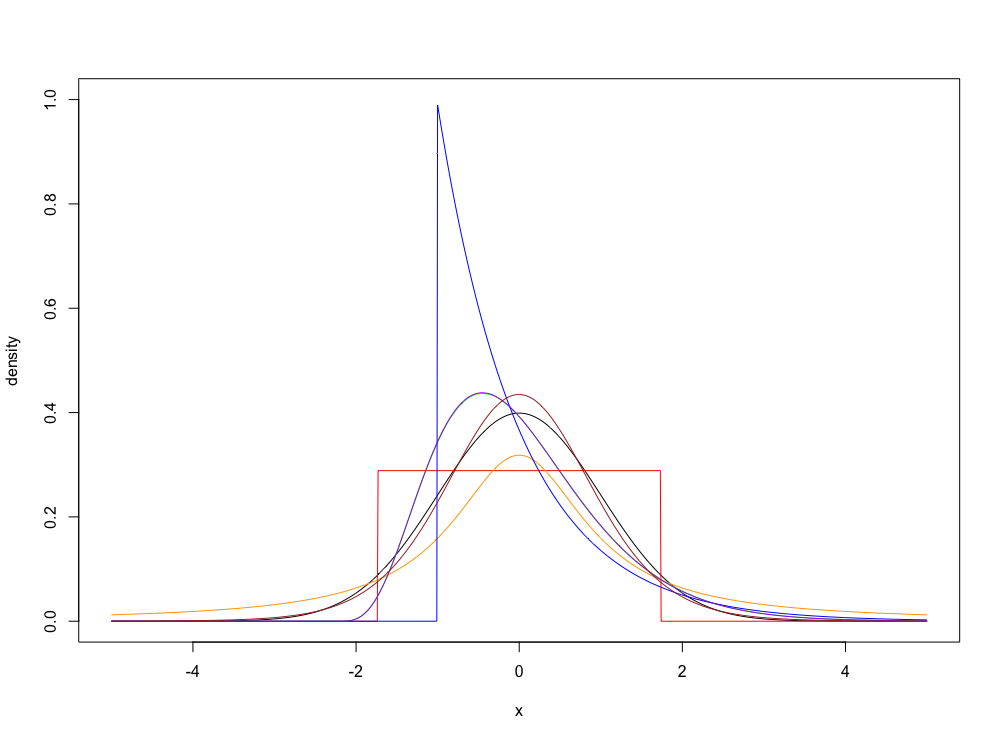
\includegraphics [height=6cm]{code/density.png}
\caption{PDF of the distributions}
\label{den}
\end{center}

We quickly report the results of Type II Error (both simulate $T=10,000$ times) in Table \ref{t2tableb} $\sim$ \ref{t2tablee}:

\begin{table}[ht]
\centering
\begin{tabular}{rrrr}
  \hline
 & n=30 & n=100 & n=1000 \\ 
  \hline
ad & \textbf{0.7028} & 0.0486 & \textbf{0.0000} \\ 
  cvm & 0.7697 & 0.1574 & \textbf{0.0000} \\ 
  lillie & 0.8589 & 0.4087 & \textbf{0.0000} \\ 
  pearson & 0.8926 & 0.5409 & \textbf{0.0000} \\ 
  sf & 0.8285 & \textbf{0.0311} & \textbf{0.0000} \\ 
   \hline
\end{tabular}
\caption{Simluation Results of Type II Error, $X\sim U(0,1)$}
\label{t2tableb}
\end{table}

\begin{table}[ht]
\centering
\begin{tabular}{rrrr}
  \hline
 & n=30 & n=100 & n=1000 \\ 
  \hline
ad & 0.0362 & \textbf{0.0000} & \textbf{0.0000} \\ 
  cvm & 0.0365 & \textbf{0.0000} & \textbf{0.0000} \\ 
  lillie & 0.0583 & \textbf{0.0000} & \textbf{0.0000} \\ 
  pearson & 0.0963 & 0.0001 & \textbf{0.0000} \\ 
  sf & \textbf{0.0307} & \textbf{0.0000} & \textbf{0.0000} \\ 
   \hline
\end{tabular}
\caption{Simluation Results of Type II Error, $X\sim \mathrm{Cauchy}(0,1)$}
\end{table}

\begin{table}[ht]
\centering
\begin{tabular}{rrrr}
  \hline
 & n=30 & n=100 & n=1000 \\ 
  \hline
ad & 0.6874 & 0.1919 & \textbf{0.0000} \\ 
  cvm & 0.7216 & 0.2625 & \textbf{0.0000} \\ 
  lillie & 0.7870 & 0.3985 & \textbf{0.0000} \\ 
  pearson & 0.8590 & 0.6090 & \textbf{0.0000} \\ 
  sf & \textbf{0.6419} & \textbf{0.1255} & \textbf{0.0000} \\ 
   \hline
\end{tabular}
\caption{Simluation Results of Type II Error, $X\sim \mathrm{Gamma}(5,3)$}
\end{table}

\begin{table}[ht]
\centering
\begin{tabular}{rrrr}
  \hline
 & n=30 & n=100 & n=1000 \\ 
  \hline
ad & 0.0638 & \textbf{0.0000} & \textbf{0.0000} \\ 
  cvm & 0.0988 & \textbf{0.0000} & \textbf{0.0000} \\ 
  lillie & 0.2170 & 0.0001 & \textbf{0.0000} \\ 
  pearson & 0.1419 & \textbf{0.0000} & \textbf{0.0000} \\ 
  sf & \textbf{0.0504} & \textbf{0.0000} & \textbf{0.0000} \\ 
   \hline
\end{tabular}
\caption{Simluation Results of Type II Error, $X\sim \mathrm{Exp}(1)$}
\end{table}

\begin{table}[ht]
\centering
\begin{tabular}{rrrr}
  \hline
 & n=30 & n=100 & n=1000 \\ 
  \hline
ad & 0.6874 & 0.1919 & \textbf{0.0000} \\ 
  cvm & 0.7216 & 0.2625 & \textbf{0.0000} \\ 
  lillie & 0.7870 & 0.3985 & \textbf{0.0000} \\ 
  pearson & 0.8590 & 0.6090 & \textbf{0.0000} \\ 
  sf & \textbf{0.6419} & \textbf{0.1255} & \textbf{0.0000} \\ 
   \hline
\end{tabular}
\caption{Simluation Results of Type II Error, $X\sim \mathcal{X}^2_{10}$}
\end{table}

\begin{table}[ht]
\centering
\begin{tabular}{rrrr}
  \hline
 & n=30 & n=100 & n=1000 \\ 
  \hline
ad & 0.8975 & 0.8349 & 0.2235 \\ 
  cvm & 0.9080 & 0.8574 & 0.3050 \\ 
  lillie & 0.9188 & 0.8894 & 0.5021 \\ 
  pearson & 0.9379 & 0.9241 & 0.8043 \\ 
  sf & \textbf{0.8486} & \textbf{0.7074} & \textbf{0.0757} \\ 
   \hline
\end{tabular}
\caption{Simluation Results of Type II Error, $X\sim T_{10}$}
\label{t2tablee}
\end{table}

We can think that the results is consistent with our intuition after seeing the plot of pdf: (except Cauchy distribution), expoential distribution is the most simple one to be distinguished. Then follows the uniform distribution, the results of Gamma(5, 3) are same with ChiSquare(10) because they are identically distributed after standardized. It might be hard to detect student's t distribution and it's curve is most similar to the curve of normal distribution.

We can draw the following conclusions:

\begin{itemize}
  \item[1.] When the significance level is fixed, Shapiro-Francia test performed best out of the five methods.
  \item[2.] Both test methods have large sample property: when $n \to \infty$, the type II error will converge to 0 (In probability or almost everywhere).
  \item[3.] It might be difficult for test to distiguish $T_\nu$ and $\mathcal{N}(0, 1)$ when $\nu$ is very large.
\end{itemize}

Here we give some plots of the large sample property of each distribution in Figure \ref{T2Eunif}, \ref{T2Ecauchy}, \ref{T2Egamma}, \ref{T2Eexp}, \ref{T2Echisq}, \ref{T2Et}

\begin{center}
\makeatletter
\def\@captype{figure}
\makeatother
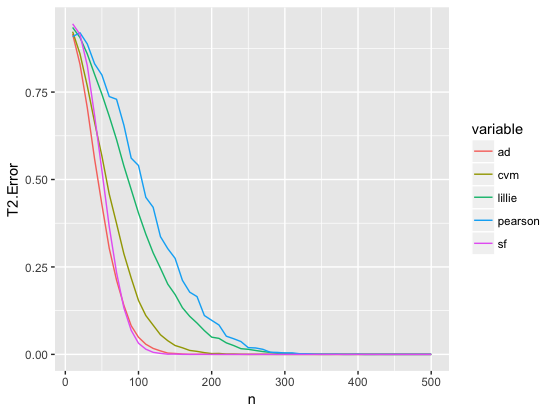
\includegraphics [height=6cm]{code/uniform.png}
\caption{Type II Error versus $n$ for $U(0,1)$}
\label{T2Eunif}
\end{center}

\begin{center}
\makeatletter
\def\@captype{figure}
\makeatother
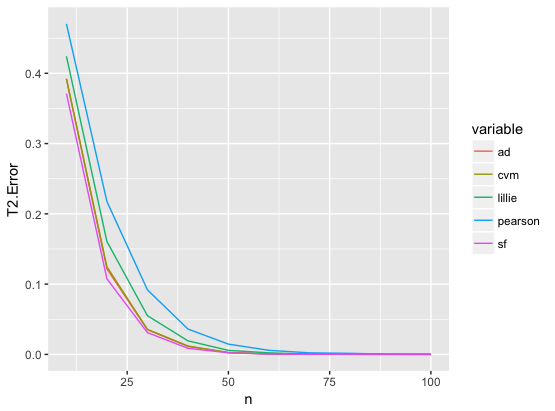
\includegraphics [height=6cm]{code/cauchy.png}
\caption{Type II Error versus $n$ for $\mathrm{Cauchy}(0,1)$}
\label{T2Ecauchy}
\end{center}

\begin{center}
\makeatletter
\def\@captype{figure}
\makeatother
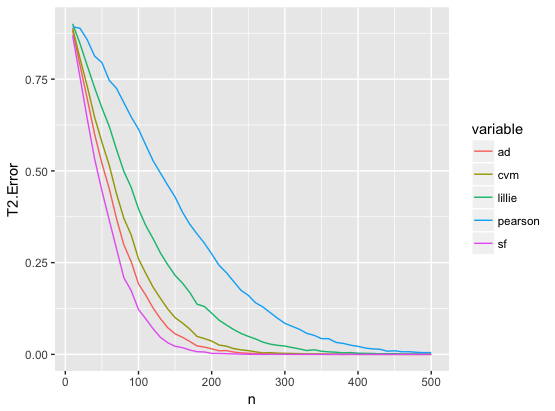
\includegraphics [height=6cm]{code/gamma.png}
\caption{Type II Error versus $n$ for $\mathrm{Gamma}(5,3)$}
\label{T2Egamma}
\end{center}

\begin{center}
\makeatletter
\def\@captype{figure}
\makeatother
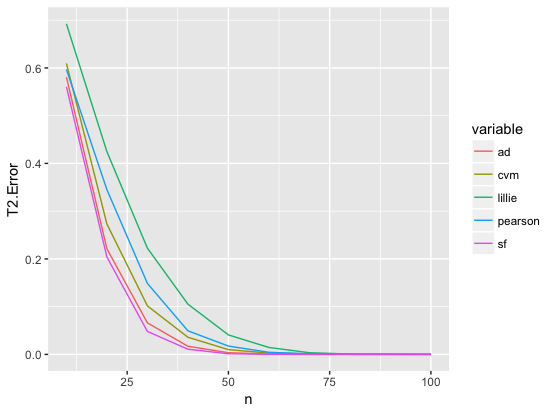
\includegraphics [height=6cm]{code/exp.png}
\caption{Type II Error versus $n$ for $\mathrm{Exp}(1)$}
\label{T2Eexp}
\end{center}

\begin{center}
\makeatletter
\def\@captype{figure}
\makeatother
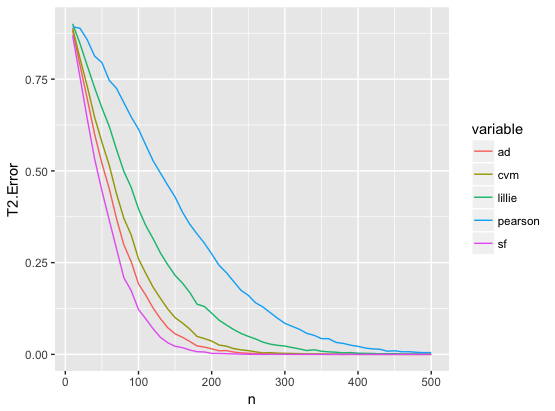
\includegraphics [height=6cm]{code/chisq.png}
\caption{Type II Error versus $n$ for $\mathcal{X}^2_{10}$}
\label{T2Echisq}
\end{center}

\begin{center}
\makeatletter
\def\@captype{figure}
\makeatother
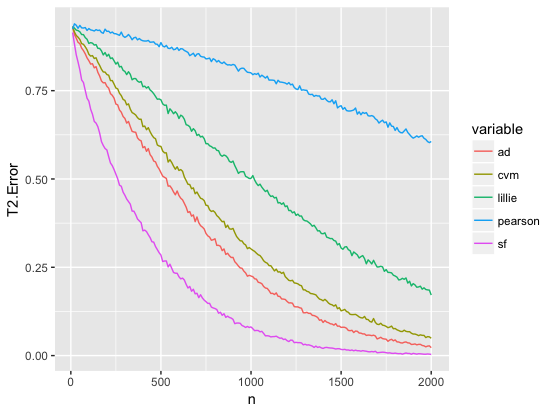
\includegraphics [height=6cm]{code/t.png}
\caption{Type II Error versus $n$ for $\sim T_{10}$}
\label{T2Et}
\end{center}

The plots give us some estimate information about number of samples we need to distinguish between other distributions and normal distribution with Type II Error is under a particular value, for example $\beta=0.05$, for SF test, We need more than 100 samples for uniform distribution, more than 40 samples for cauchy distribution, more than 150 samples for $\mathrm{Gamma}(\alpha=5)$, more than 38 samples for exponential distribution, more than 1600 samples for $T_{10}$.

\subsection{Mixture normal distribution}

We generate data from the population with pdf $f(x)=\pi \varphi(x) + (1-\pi) \varphi((x-\mu)/\sigma)$, where $\varphi(x)$ is the pdf of $\mathcal{N}(0,1)$. We can then regard the original hypothesis testing as a parametric hypothesis testing, with null hypothesis $\pi=0$ and alternative hypothesis $\pi \in (0,1/2]$. 

Here we let $\mu=5, \sigma=1$ and change $\pi$, then plot the power function for all the methods for $n=30$, $n=100$ and $n=1000$ in Figure \ref{m.pf30}, \ref{m.pf100} and \ref{m.pf1000}

\begin{center}
\makeatletter
\def\@captype{figure}
\makeatother
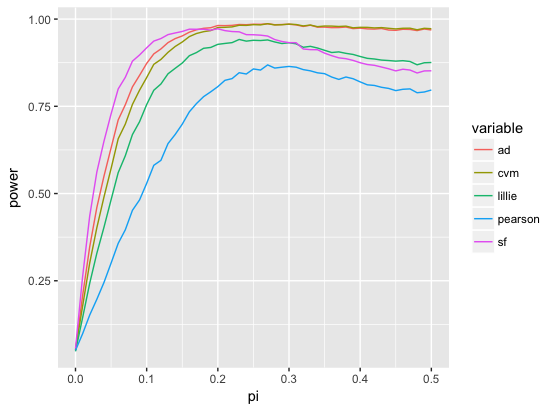
\includegraphics [height=6cm]{code/mixture.30.png}
\caption{Power function with mixture normal population, $n=30$}
\label{m.pf30}
\end{center}

\begin{center}
\makeatletter
\def\@captype{figure}
\makeatother
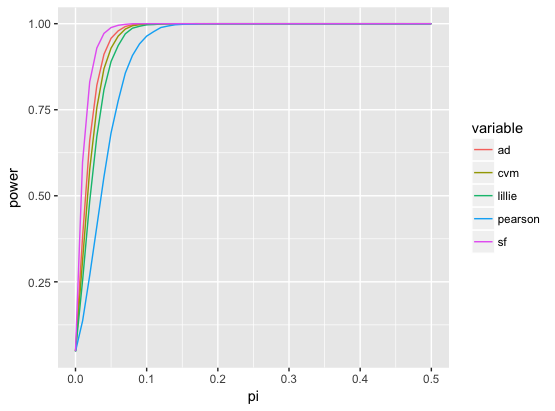
\includegraphics [height=6cm]{code/mixture.100.png}
\caption{Power function with mixture normal population, $n=100$}
\label{m.pf100}
\end{center}

\begin{center}
\makeatletter
\def\@captype{figure}
\makeatother
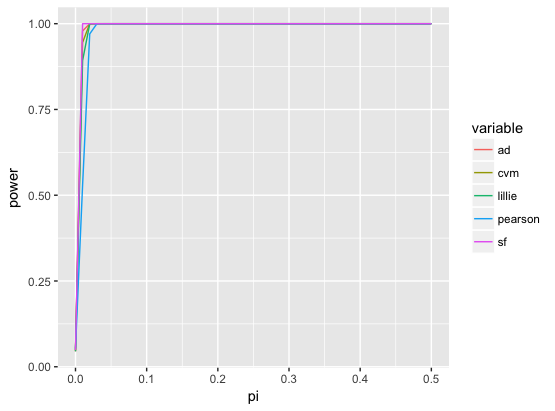
\includegraphics [height=6cm]{code/mixture.1000.png}
\caption{Power function with mixture normal population, $n=1000$}
\label{m.pf1000}
\end{center}

We can see that SF test outperform other methods when $n=100$ and $n=1000$, which has the largest power. However, when $n=30$ and $\pi \ge 0.2$ we can see the power decreases for lillie, pearson and sf method.

\subsection{Student's t Approximation}

Since the pdf of the Students's t distribution is

\begin{eqnarray}
f(t) = \frac{\Gamma(\frac{\nu+1}{2})} {\sqrt{\nu\pi}\,\Gamma(\frac{\nu}{2})} \left(1+\frac{t^2}{\nu} \right)^{\!-\frac{\nu+1}{2}}
\end{eqnarray}

We can see that when $\nu\to \infty$, the term which contains $t$ will coverge to $e^{-t^2/2}$, which approximate the form of normal distribution. When we regard $\nu$ as parameter, the original hypothesis testing could become a parametric hypothesis testing, therefore can easily plot the power function can evaluate its property. We assume that when $\nu$ is very large, the samples are sampling from normal distribution.

We plot the power function for all the methods for $n=30$, $n=100$ and $n=1000$ in Figure \ref{t.pf30}, \ref{t.pf100} and \ref{t.pf1000}

\begin{center}
\makeatletter
\def\@captype{figure}
\makeatother
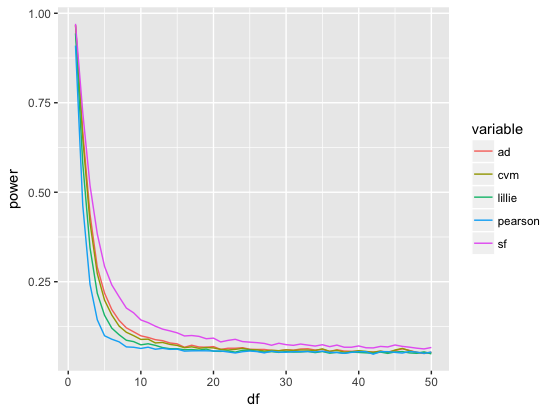
\includegraphics [height=6cm]{code/t.30.png}
\caption{Power function with population $T_\nu$, $n=30$}
\label{t.pf30}
\end{center}

\begin{center}
\makeatletter
\def\@captype{figure}
\makeatother
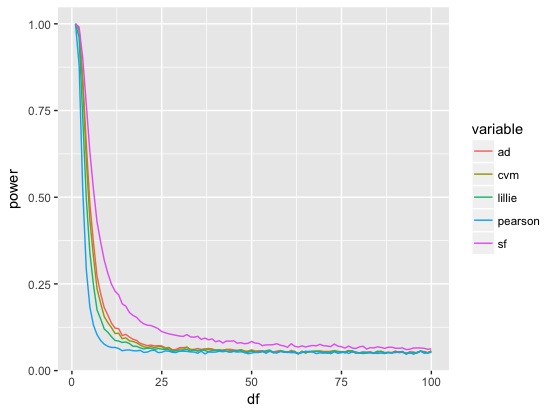
\includegraphics [height=6cm]{code/t.100.png}
\caption{Power function with population $T_\nu$, $n=100$}
\label{t.pf100}
\end{center}

\begin{center}
\makeatletter
\def\@captype{figure}
\makeatother
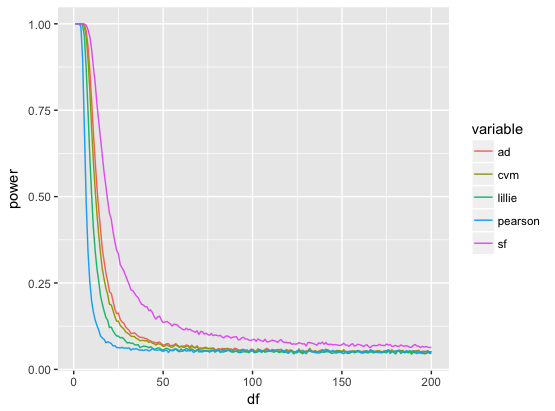
\includegraphics [height=6cm]{code/t.1000.png}
\caption{Power function with population $T_\nu$, $n=1000$}
\label{t.pf1000}
\end{center}

We can see that SF test outperform other methods, which has the largest power.

\subsection{Intrisic Error}

We firstly sample $Y$ from $\mathcal{N}(0, 1)$ and use transform $X=Y+\epsilon\sin(Y)$ to generate data $X$. We can also regard the original hypothesis testing as a parametric hypothesis testing, with null hypothesis $\epsilon=0$ and alternative hypothesis $\epsilon \in (0,1]$. 

We plot the power function for all the methods for $n=30$, $n=100$ and $n=1000$ in Figure \ref{i.pf30}, \ref{i.pf100} and \ref{i.pf1000}

\begin{center}
\makeatletter
\def\@captype{figure}
\makeatother
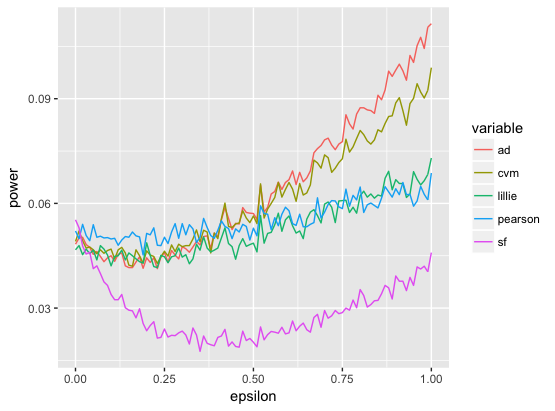
\includegraphics [height=6cm]{code/noise.30.png}
\caption{Power function with tranformed population $X=Y+\epsilon\sin(X)$, $n=30$}
\label{i.pf30}
\end{center}

\begin{center}
\makeatletter
\def\@captype{figure}
\makeatother
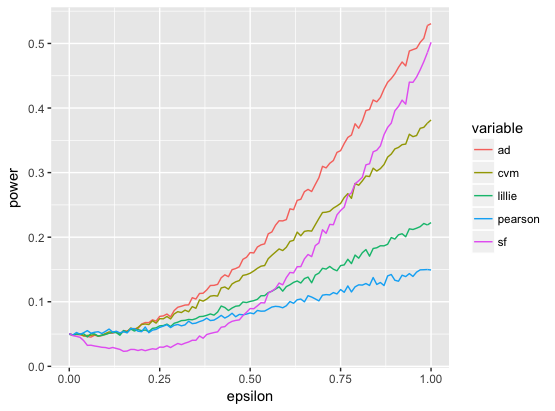
\includegraphics [height=6cm]{code/noise.100.png}
\caption{Power function with tranformed population $X=Y+\epsilon\sin(X)$, $n=100$}
\label{i.pf100}
\end{center}

\begin{center}
\makeatletter
\def\@captype{figure}
\makeatother
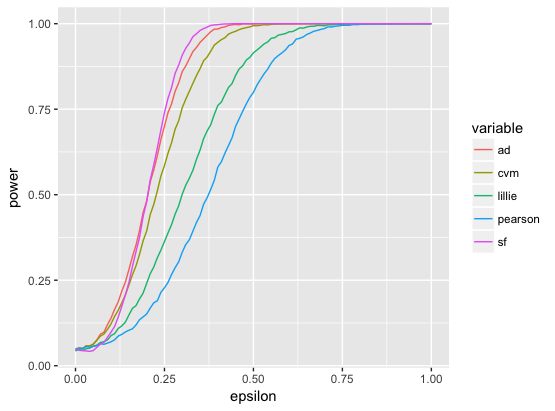
\includegraphics [height=6cm]{code/noise.1000.png}
\caption{Power function with tranformed population $X=Y+\epsilon\sin(X)$, $n=1000$}
\label{i.pf1000}
\end{center}

Also, when $n$ becomes larger, all methods become better, when $n=1000$, SF test becomes the best. When $n=30$ and $n=100$, SF test don't perform well and AD test might be better.

\end{document}
